%% The following is a directive for TeXShop to indicate the main file
%%!TEX root = diss.tex

\chapter{Discussion and conclusions}
\label{chap:conclusion}

This dissertation has examined the influence of attentional sets on perceptual learning in speech perception.
Through explicit instructions and experimental manipulations, listeners were induced towards a more comprehension-oriented attentional set or a more perception-oriented attentional set.
Those participants in conditions biased towards comprehension showed larger perceptual learning effects than those in conditions biased more towards perception.
I adopted a predictive coding framework \citep{Clark2013} that provides an intuitive model of perceptual learning and has been computationally implemented \citep{Kleinschmidt2011}.
However, the attentional mechanism in the predictive coding framework does not work well for some instances of visual attention \citep{Block2013}, or for the current results.
I propose a new attentional mechanism for predictive coding, one in which attention inhibits error propagation beyond the level to which attention is directed.  Such a mechanism explains both the previous findings and the current results.

\begin{figure*}[!ht]
\centering
\caption{Distribution of crossover points for each participant across all experiments.  Dashed line represents the midpoint of the continua.}
\label{fig:exp123xoverdist}
\begin{center}
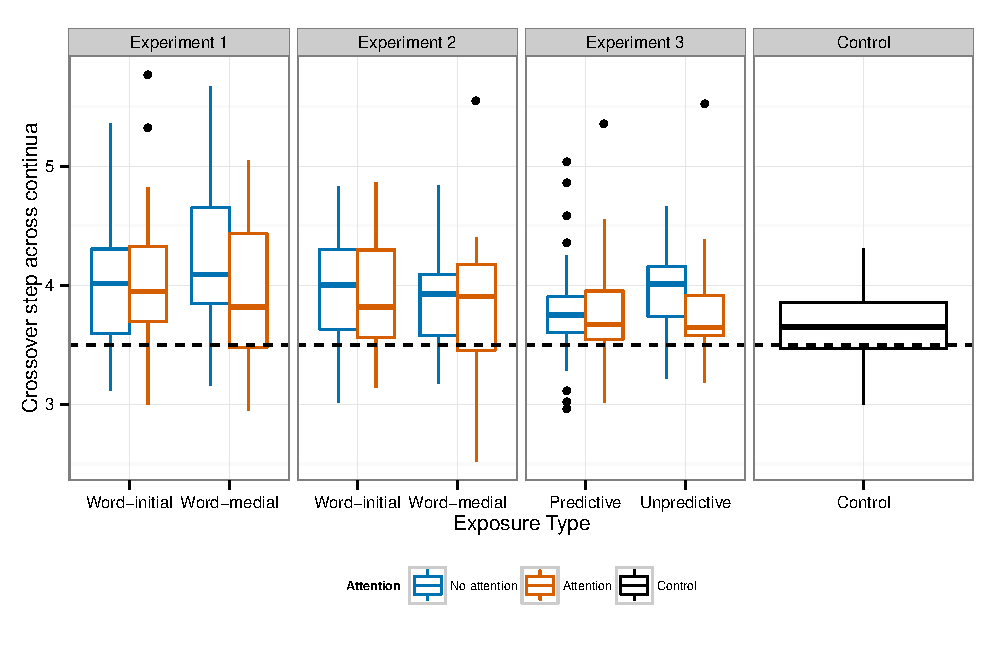
\includegraphics[width=0.9\textwidth]{graphs/exp123_xoverdist}
\end{center}
\end{figure*}


\section{Attentional control of perceptual learning}

The findings of Experiment 1 support the hypothesis that comprehension-oriented attentional sets produce larger perceptual learning effects than perception-oriented attentional sets.  
Although all participants showed perceptual learning effects, those exposed to the ambiguous sound with increased lexical bias only showed larger perceptual learning effects when the instructions about the speaker's ambiguous sound were withheld.  
Attention on the ambiguous sound equalized the perceptual learning effects across lexical bias.
However, in Experiment 2, there is no such effect of attention, suggesting that the ambiguous sounds that were farther away from the canonical production induced a more perception-oriented attentional set.

One question raised by the current results is whether perception-oriented attentional sets always result in decreased perceptual learning.  
The instructions used to focus the listener's attentional set framed the ambiguity in a negative way, with listeners being cautioned to listen carefully to ensure they made the correct decision.  
If the attention were directed to the ambiguous sound by framing the ambiguity in a positive way, would we still see the same pattern of results?
The current mechanism would predict that attention of any kind to signal properties would block the propagation of errors, reducing perceptual learning.
This prediction will be tested in future work.

\section{Specificity versus generalization in perceptual learning}

The results of this dissertation speak to dichotomy between specificity and generalization found in perceptual learning work. 
In Experiment 1, greater perceptual learning was shown by participants exposed to ambiguous sounds later in the words, not to those at the beginnings of words. 
And yet, the testing continua consisted of stimuli with the sibilant at the beginnings of words, which are more similar to the words beginning with the ambiguous sound.
In this sense, there was not only a lack of exposure-specificity, but a level of abstraction that is usually not assumed in perceptual learning studies.
Most lexically-guided perceptual learning studies attempt to make the exposure tokens and the categorization as similar, and in some cases, the same, in order to maximize exposure-specificity effects.
The results of this dissertation show that not only do listeners show perceptual learning effects from stimuli with large degrees of coarticulation (i.e., in the middle of the word) to stimuli without as much coarticulation, in some cases, perceptual learning is enhanced in precisely those cases.

The effect of attentional set manipulations in Experiments 1 and 2 suggest that when listeners adopt more perceptually-oriented attentional sets, even within tasks that are oriented toward comprehension, generalization of perceptual learning to new forms is inhibited.
While visually-guided perceptual learning shows comparable effects to lexically-guided perceptual learning \citep{vanLinden2007}, lexically-guided perceptual learning is more likely to be expanded to new contexts \citep{Norris2003, Kraljic2008a}, though with some restrictions \citep{Mitterer2013}, than visually-guided perceptual learning \citep{Reinisch2014}.
Visually-guided and psychophysical perceptual learning paradigms often have highly repetitive stimuli with little variation.  
Both of these aspects add to the monotony and the likelihood of perception-oriented attentional sets \citep{Cutler1987}.
Lexically-guided perceptual learning, on the other hand, requires very few instances to affect the perceptual system, usually around 20 ambiguous tokens within 200 trials, but as few as 10 ambiguous tokens have been shown to have comparable effects \citep{Kraljic2008}.
Following from the proposed attention mechanism, tokens heard under a comprehension-oriented attentional set should have a relatively large effect on the perceptual system as compared to tokens heard under a perception-oriented attentional set.
This prediction is borne out by the lack of correlation between word endorsement rate and crossover point in Experiment 1 in the Word-final/No attention condition.
This condition is predicted to have the most comprehension-oriented attentional set of the conditions, and here is the only instance in Experiment 1 where a strong correlation between word endorsement rate and crossover point is not present.
Participants in this condition have relatively high crossover points that do not depend as much on the sheer number of tokens endorsed.

\section{Effect of increased linguistic expectations}

In comparing Experiments 1 and 3, increasing linguistic expectations does not increase perceptual learning.  
While the Isolation condition (Word-medial condition in Experiment 1) was not significantly different from the Unpredictive condition of Experiment 3, the trend was reduced perceptual learning when the modified sound category was embedded in a sentential context.
The Predictive condition showed significantly less perceptual learning than the Isolation condition, but this could be driven by the wide variability found in that condition, as shown in Figure~\ref{fig:exp123xoverdist}.
Sentence processing may be too comprehension-oriented, and a balance between comprehension and perception is necessary for perceptual learning to be generalized.

Several studies have shown perceptual learning benefits for multiple talkers of an accent using sentential stimuli \citep[and others]{Bradlow2008}.  
Clearly, perceptual learning of accents is possible through hearing sentences, but the variability involved in those tasks reaches far beyond that involved here.  
The speaker producing the sentences in this dissertation is a native English speaker.
Even with the synthesis applied to the sound files, he is likely more intelligible than the speakers in studies involving foreign accents.
The ease of comprehension of the speaker in this study might actually inhibit perceptual learning in sentences, because listeners can leverage so much of their perceptual experience with other speakers of the local dialect.

\section{Category atypicality}

In Experiment 2, there was no effect of explicit instructions or lexical bias on perceptual learning, with a stable perceptual learning effect present for all listeners.
There are two potential, non-exclusive explanations for the lack of effects.
As stated above, the increased distance to the canonical production drew the listener's attention to the ambiguous productions, resulting in a perception-oriented attentional set.
The second potential explanation is that the productions farther from canonical produce a weaker effect on the updating of a listener's categories, as predicted from the neo-generative model in \citep{Pierrehumbert2002}.
This explanation is supported in part by the weaker correlation between word endorsement rate and crossover point found in Experiment 2, and the findings of \citet{Sumner2011} where the most perceptual learning was found when the categories begin like the listener expects and gradually shift toward the speaker's actual boundaries over the course of exposure.
This explanation could be tested straightforwardly by implementing the same gradual shift paradigm used in \citet{Sumner2011} with the manipulations used in this dissertation.

An interesting extension to the current findings would be to observe the perceptual learning effects in a cognitive load paradigm.  Speech perception under cognitive load has shown to have greater reliance on lexical information due to weaker initial encoding of the signal \citep{Mattys2011}.  Following exposure to a modified ambiguous category, we might expect to see less perceptual learning if the exposure was accompanied by high cognitive load.  However, \citet{Scharenborg2014} found that hearing loss of older participants did not significantly influence their perceptual learning.  Therefore it may be that perceptual learning would likewise be similar across cognitive loads.
Higher cognitive loads, however, might allow for more atypical ambiguous stimuli to be learned, due to the increased reliance on lexical information during initial encoding.

It is important to bear in mind that what is typical in one context is not necessarily typical in another.  
The methodology employed for Experiment 3 drew on the assumptions that variance would common between the Experiments.  
However, it may be that the perfectly ambiguous /s/ category in Experiment 3 was within the range of variation when a word is predicted from context. 
In this case, had the category atypicality been more like that of Experiment 2, we may have actually seen more of an effect, perhaps back to the level of Experiment 1.

\section{Conclusion}

This dissertation investigated the influences of attention and linguistic salience on perceptual learning in speech perception.
Perceptual learning was modulated by the attentional set of the listener.
Decreased linguistic salience by increasing linguistic expectations induced more comprehension-oriented attentional sets, resulting in larger perceptual learning effects.
Inducing perception-oriented attentional sets through explicit instructions or making the modified sound category more atypical resulted in smaller perceptual learning effects.
These results support a greater role of attention than previously assumed in predictive coding frameworks, such as the proposed propagation-blocking mechanism.
Finally, these results suggest that the degree to which listeners perceptually adapt to a new speaker is under their control to a degree, but given the robust perceptual learning effects across all conditions, perceptual learning is a largely automatic process.


